\chapter{Space Segment}

\section{Overview}

One or more spacecraft make up the space segment. A spacecraft is composed of one or more payloads, and the spacecraft bus, also called platform. The platform is in turn composed of a number of subsystems that each provide some functional aspect for supporting the payload operations.

\section{Payload}

The payload system provides the functionality to fulfill the specific mission objectives. For earth observation mission the payloads may be optical cameras or other remote sensing instruments. For communications mission the payload may be a transponder. For science missions the payload may be a certain type of novel instrument. With such a variety of mission objectives the standardization of payloads on system level is an unrealistic approach. On the other hand, what can be standardized to some extended is the interfaces to it, and possibly some of its onboard data processing.

\subsection{Data Compression}

\subsubsection{Lossless Data Compression}

\begin{tabular}{l}
\textit{CCSDS-121.0-B "Lossless Data Compression" \cite{CCSDS-120.0-G}} \\
\textit{CCSDS-120.0-G "Lossless Data Compression" \cite{CCSDS-121.0-B}}
\end{tabular}

The lossless source coding technique preserves source data accuracy and removes redundancy in the data source. This technique is particularly useful when data integrity cannot be compromised. The described lossless source coder consists of two separate functional parts: the preprocessor and the adaptive entropy coder. 

The role of the \textbf{preprocessor} is to transform the data into samples that can be more efficiently compressed by the entropy encoder. It applies a reversible function to input data samples to produce the lowest entropy, which is a measure of the smallest average number of bits that can be used to represent each sample. In general a preprocessor that removes correlation between samples in the input data block will improve the performance of the entropy coder. The \textbf{adaptive entropy coder} uses variable-length codes and compresses data by assigning shorter codewords to symbols that are expected to occur with higher frequency. By using several different codes and transmitting the code identifier, the algorithm can adapt to many sources from low entropy (more compressible) to high entropy (less compressible).

\begin{tabular}{l}
\textit{CCSDS-123.0-B "Lossless Multispectral and Hyperspectral Image Compression" \cite{CCSDS-123.0-B}}
\end{tabular}

The described compressor is applicable to three-dimensional arrays of integer sample values (as obtained from multispectral and hyperspectral imagers and sounders). It consists of two functional parts: a predictor and an encoder. The \textbf{predictor} has as input the original image data and predicts the value of each image sample based on the values of nearby samples in a small three-dimensional neighbourhood. These mapped predictions make up the predictor output. The \textbf{encoder} then works similar as the adaptive entropy encoder presented above, using statistical data that is updated after each sample is encoded.

\subsubsection{Lossless and Lossy Image Data Compression}

\begin{tabular}{l}
\textit{CCSDS-122.0-B "Image Data Compression" \cite{CCSDS-122.0-B}} \\
\textit{CCSDS-120.1-G "Image Data Compression" \cite{CCSDS-120.1-G}}
\end{tabular}

Several lossless and lossy image compression algorithms are widely used, such as JPEG2000 and JPEG-LS. This standard however describes a fast and less complex algorithm that can be applied to greyscale images with integer-valued pixels with a bit depth of 16 bits. It consists of two functional parts: a discrete wavelet transform and a bit-plane encoder. The \textbf{discrete wavelet transform} performs low-pass and high-pass filtering along first horizontal and then vertical direction, resulting in four subband data arrays, each half as wide and half as tall as the original image array. This step is repeated two more time, each time with the obtained left upper subband data array as input. This produces a total of 10 subbands. The \textbf{bit-plane encoder} then processes 64 wavelet coefficients, which are made up from the 16 equally sized blocks of the most upper left subband (termd the DC coefficients) and their mapping to the other subbands.

\subsubsection{Digital Motion Imagery}

\begin{tabular}{l}
\textit{CCSDS-766.1-B "Digital Motion Imagery" \cite{CCSDS-766.1-B}} \\
\textit{CCSDS-706.1-G "Motion Imagery and Applications" \cite{CCSDS-706.1-G}}
\end{tabular}

This standard categories different video applications and relates to it appropriate video resolutions and frame rates. It specifies the commonly used MPEG-4 Part 10 (H.264) as the encoding format intended for real-time applications where live, or nearly live, video needs to be monitored at a ground location during an event or experiment. Further, JPEG2000 is intended for requirements for higher quality or where each individual frame needs to be maintained intact. 

\section{Platform}

\subsection{Mechanical}

\subsubsection{Structure}

\begin{tabular}{l}
\textit{"CubeSat Design Specification" \cite{cubesat_design_specification}}
\end{tabular}

The main purpose of the CubeSat design specification (CDS) is to ensure that CubeSats can fit inside a deployment system, of which California Polytechnic State University's P-POD (Poly Picosatelite Orbital Deployer) sets the standard, and to ensure that the CubeSat does not pose a threat to neighboring payloads. While the specification's main focus is on the definition of the mechanical outline of the primary structure and its geometrical properties, it also includes requirements on the material to be used and its surface finish. The original CDS introduced the cubic shaped 10x10x10 cm$^{3}$ single unit (1U) CubeSat design (as shown in Figure \ref{fig:1U CubeSat Design Specification Drawing}), however now the specification also includes definitions for multiples thereof (e.g. 1.5U, 2U, 3U, 3U+).

\begin{figure}[h]
\centering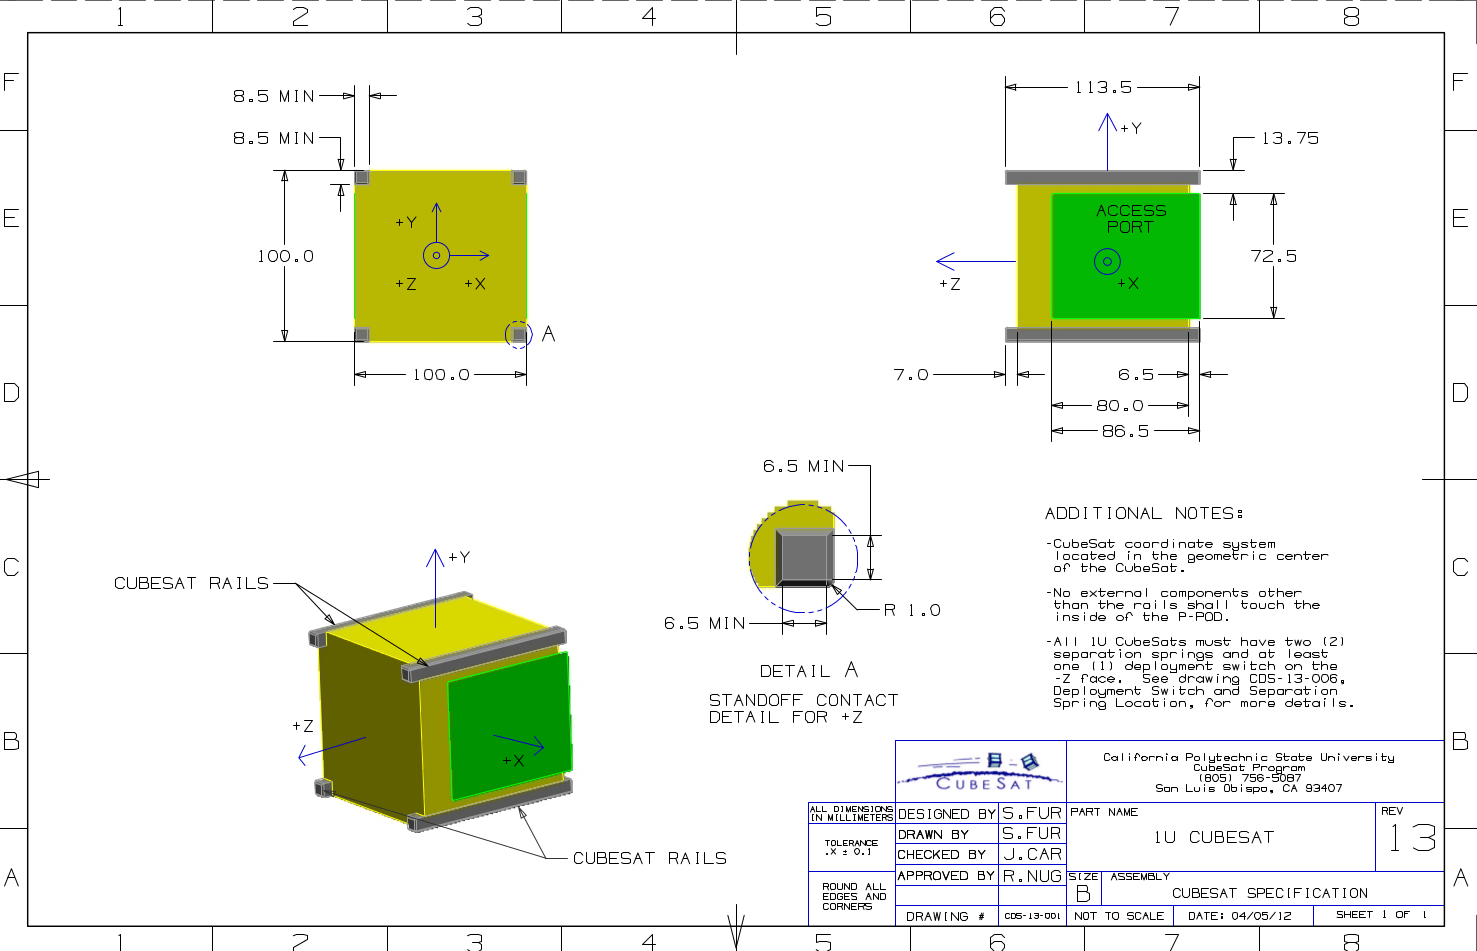
\includegraphics[scale=0.25]{fig/1u_cubesat_design_specification_drawing}
\caption{1U CubeSat Design Specification Drawing}
\label{fig:1U CubeSat Design Specification Drawing}
\end{figure}

\subsubsection{Mechanisms}

\begin{tabular}{l}
\textit{"CubeSat Design Specification" \cite{cubesat_design_specification}}
\end{tabular}

The design of mechanisms is very much mission specific. Deployments from CubeSats, such as booms or wires, have not reached a sufficient maturity that even a best practises could be derived. The exception to this is the definition of two mechanisms that part of the CubeSat specification: separation springs and deployment switches. Usually several CubeSats are launched inside a single deployer. The purpose of the \textbf{separation springs} is then to ensure adequate separation of CubeSats when ejected from the deployer. They are for obvious reasons not required on CubeSats that are contained in equally sized deployment containers. The purpose of the \textbf{deployment switches} is to completely power-off the CubeSat during launch while inside the deployer. The two separation springs and two deployment switches shall be integrated at the four rails on the -Z facing end and shall be diagonal to each other.  

\subsection{Electrical}

\subsubsection{Power Distribution Switches}

\begin{tabular}{l}
\textit{ECSS-E-ST-20-20 "Electrical design and interface requirements for power supply" \cite{ECSS-E-ST-20-20}} \\
\textit{ECSS-E-HB-20-20 "Guidelines for electrical design and interface requirements for power supply" \cite{ECSS-E-HB-20-20}} \\
\end{tabular}

Two types of power distribution switches are available. The \textbf{latching current limiter} (LCL) is a switchable and latching protection between a power source and the load, causing a trip off after having achieved at its outputs and over-current limitation for a defined trip-off time (Figure \ref{fig:LCL Generic Block Diagram}). In case of a load malfunction implying an overload, they enter current limitation mode for the given trip off time duration, and then switch off. LCLs can be externally commanded into ON or OFF mode.

The \textbf{retriggerable latching current limiter} (RLCL) is an LCL that automatically attempts to switch ON when powered or after a retrigger interval when a trip off event occurred. RLCLs are normally used to supply essential spacecraft loads (for example decoders, receivers, and reconfiguration modules) and as such they are supposed to provide continuously power to the load after start up. They react similar to a load malfunction, namely to limit current and then switch off. But they will attempt a re-start automatically after a defined time duration.

\begin{figure}[h]
\centering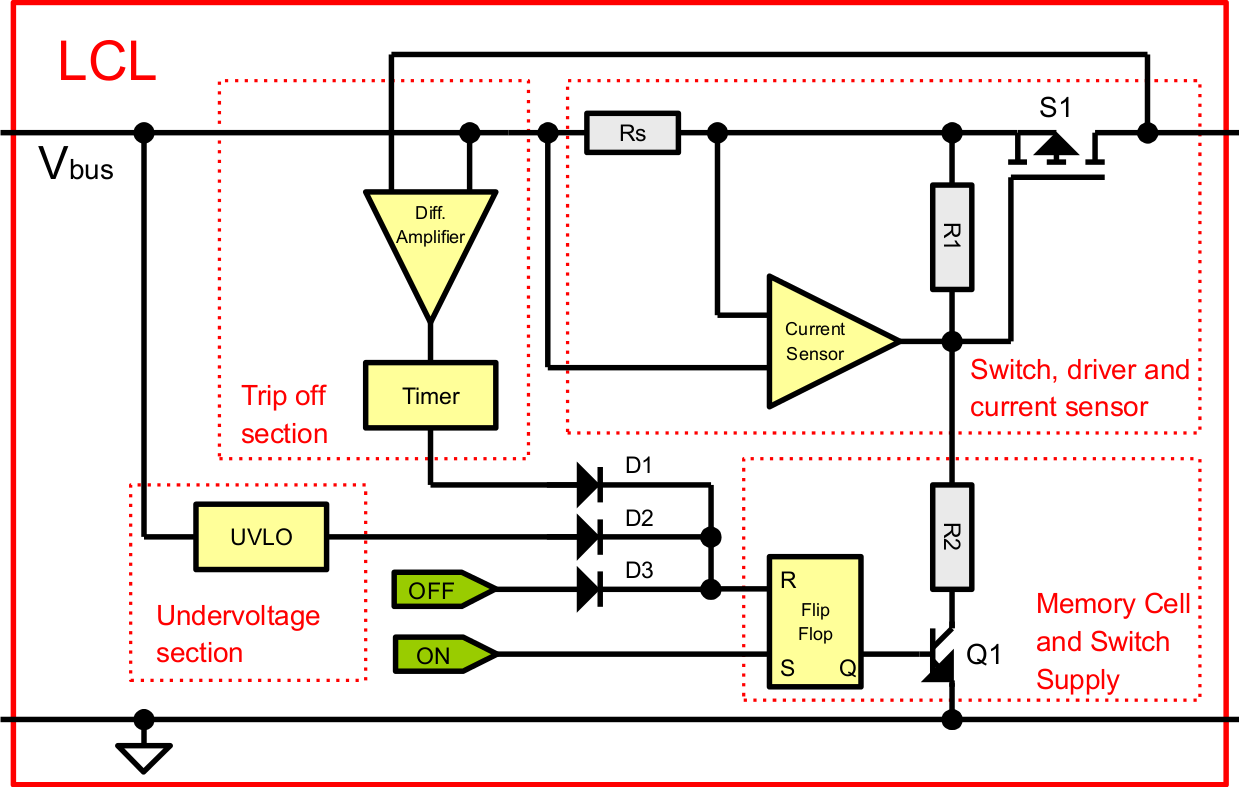
\includegraphics[scale=0.2]{fig/lcl_generic_block_diagram}
\caption{LCL Generic Block Diagram}
\label{fig:LCL Generic Block Diagram}
\end{figure}

\subsubsection{Discrete Interfaces}

\begin{tabular}{l}
\textit{ECSS-E-ST-50-14 "Spacecraft discrete interfaces" \cite{ECSS-E-ST-50-14}} \\
\end{tabular}

Discrete interfaces are used typically for sensor acquisition and actuator control. These interfaces can be broadly categorized into the following types: analog, bi-level digital, pulse commands, and serial digital interfaces. For units that are to be used in redundancy, the driver and receiver interfaces are to be cross-strapped as shown in Figure \ref{fig:General Scheme of Cross-Strapping}.

\begin{figure}[h]
\centering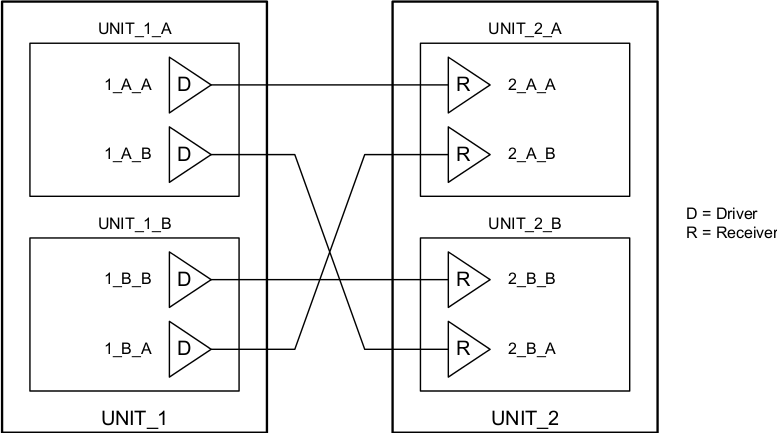
\includegraphics[scale=0.4]{fig/general_scheme_of_cross_strapping}
\caption{General Scheme of Cross-Strapping}
\label{fig:General Scheme of Cross-Strapping}
\end{figure}

The \textbf{analog signal interfaces} are used for direct connection to a device which produces a continuous variable analog voltage to indicate the value of the parameter being measured. Usually, the analog voltage produced by the sensor or a peripheral element is converted into a digital value within the element to which it is connected. The basic application scenario is a differential voltage range from 0 to 5 V with a signal bandwidth of up to 1 Hz (i.e. a slowly changing, quasi-static signal) and a conversion resolution of 12 bits.

A special case of analog signals are \textbf{temperature sensors} (thermistors). These are resistors that change resistance with temperature, either with the temperature gradient (positive temperature coefficient, PTC) or opposite (NTC). Figure \ref{fig:Temperature Sensor Interface Arrangement} shows a typical temperature sensor interface arrangement.

\begin{figure}[h]
\centering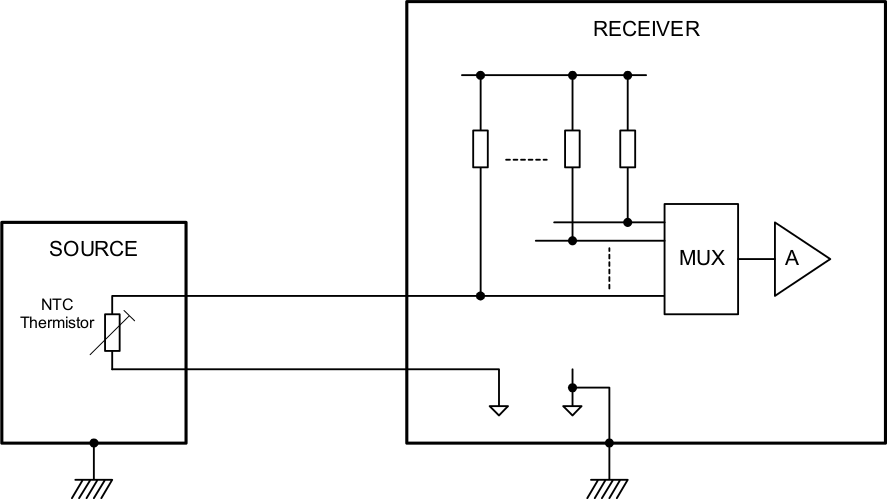
\includegraphics[scale=0.3]{fig/temperature_sensor_interface_arrangement}
\caption{Temperature Sensor Interface Arrangement}
\label{fig:Temperature Sensor Interface Arrangement}
\end{figure}

The \textbf{digital signal interfaces} are used for signals that take only two values, high or low, indicated by the signal voltage. Typically the low voltage ranges from 0 to 0.9 V and high voltage from 2.0 to 5.5 V for a 5 V interface. The signal sources are high impedance, meaning that they carry only a small current in the order of micro- or milliampere. Note that a number of such interfaces can be arranged in parallel to form an arrangement for transmission of larger data words and associated clock and read/write control capabilities.

The \textbf{pulsed command interfaces} on the other hand are intended for load driving interfaces and, for example, can be used to switch relays or similar loads. They provide high current capabilities in the order of up to 1 Ampere. A typical high power commanding interface arrangement is shown in Figure \ref{fig:High Power Commanding Interface Arrangement}.

\begin{figure}[h]
\centering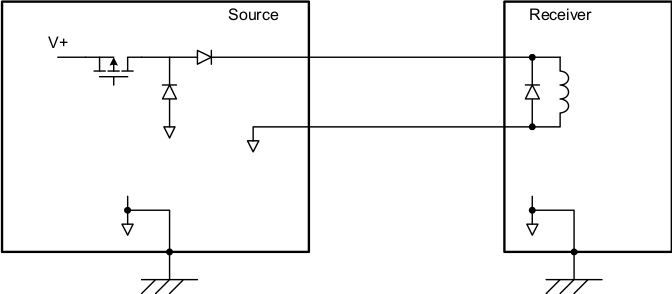
\includegraphics[scale=0.3]{fig/high_power_commanding_interface_arrangement}
\caption{High Power Commanding Interface Arrangement}
\label{fig:High Power Commanding Interface Arrangement}
\end{figure}
 
The \textbf{serial digital interfaces} for point-to-point communication are used to exchange digital data words between core and peripheral elements. Typically universal asynchronous receiver/transmitter (UART) are used for that. It takes bytes of data and transmits the individual bits in a sequential fashion. At the destination, a second UART re-assembles the bits into complete bytes. The UART usually does not directly generate or receive the external signals used between different items of equipment. Separate interface devices are used to convert the logic level signals of the UART to and from the external signaling levels. External signals may be of many different forms. Common microcontrollers support the RS-232 specification that is also known as the serial port on computers. The RS-422 is similar to it but provides for differential signal levels and hence requires two lines per transmit/receive signal. In both cases an intermediate circuit element is needed to convert from CMOS/TTL levels coming from the microcontroller to the larger voltage levels required by the RS-232/RS-422 specification.
 
\subsubsection{Data Bus}

\begin{tabular}{l}
\textit{ECSS-E-ST-50-15 "CANbus extension protocol" \cite{ECSS-E-ST-50-15}} \\
\end{tabular}

Data buses are used for spacecraft on-board communications and control. Typically the data rates are moderate, as they are intended to route telecommands and telemetry, but usually are not indented for streaming science or other high-volume data. The main objective of the data bus is to be highly reliable.

The CAN (Controller Area Network) bus has been successfully used in automotive and critical control industry for more than three decades. The ECSS-CAN standard specifies the requirements for the use of CAN data bus in spacecraft onboard applications. They extend the CAN network specification to cover aspects of the physical and data link layer related to the particular needs of spacecraft data handling systems. 

CAN is by itself a multi-master network, so each node may send messages at any time. Collisions get resolved by message priority. For this to work, each CAN message identifiers used in a network must be unique. A CAN network is composed of two or more nodes. Each of these nodes (see Figure \ref{fig:CAN Bus Node}) include a central processing unit (such as microcontroller), a CAN controller (often integrated in microcontroller), and a CAN transceiver. 

\begin{figure}[h]
\centering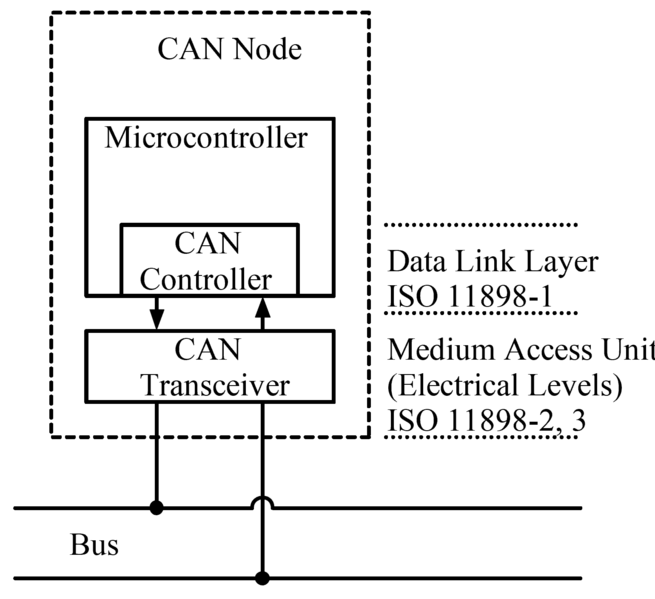
\includegraphics[scale=0.3]{fig/can_bus_node}
\caption{CAN Bus Node}
\label{fig:CAN Bus Node}
\end{figure}

CAN may be implemented on different physical transmission media like twisted pair, power lines, optical and others. A CAN transceiver is used to connect the CAN controller and the physical medium. The transceiver takes the TTL (or CMOS) signal from the controller’s transmit pin and converts it to a differential signal between the two wires of the network cable. In return, differential signals on the two wires of the network cable are converted back into TTL/CMOS level and fed back to the controller’s receive pin.

The data link layer represents the kernel of the CAN protocol. It is responsible for bit timing and synchronization, message framing, arbitration, acknowledgement, error detection and signaling, and fault confinement.

The CAN standard does not include tasks of application layer protocols, such
as flow control, device addressing, and transportation of large data blocks. Many
implementations of higher layer protocols were created to address those issues. The CANopen specification is one of the most widespread protocol stack for industrial applications and has been adopted for the ECSS-CAN bus extension protocol as optional for use as an application layer protocol. 

CANopen is a communication protocol and device profile specification for embedded systems used in automation. In terms of the OSI (Open Systems Interconnection) model, CANopen implements the layers above and including the network layer. The CANopen standard consists of an addressing scheme, several small communication protocols and an application layer defined by a device profile (see Figure \ref{fig:CANopen Device Model}). The communication protocols have support for network management, device monitoring and communication between nodes, including a simple transport layer for message segmentation/desegmentation.

\begin{figure}[h]
\centering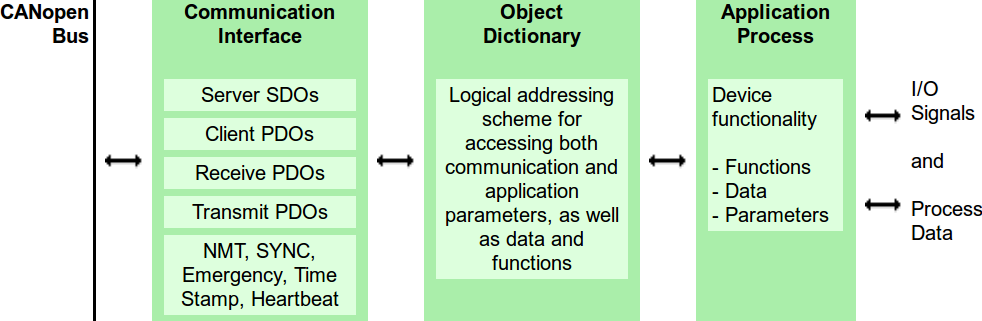
\includegraphics[scale=0.4]{fig/canopen_device_model}
\caption{CANopen Device Model}
\label{fig:CANopen Device Model}
\end{figure}


\subsection{Attitude and Orbit Control}

\subsubsection{Sensors}

\begin{tabular}{l}
\textit{ECSS-E-ST-60-20 "Stars sensors terminology and performance specification" \cite{ECSS-E-ST-60-20}} \\
\end{tabular}

This standard defines the terminology and specification definitions for the performance of star trackers (in particular, autonomous star trackers). It focuses on the specific issues involved in the specification of performances of star trackers and is intended to be used as a structured set of systematic provisions. The standard defines and normalizes terms used in star sensor performance specifications, as well as some performance assessment conditions:

\begin{itemize}
\item Sensor components
\item Sensor capabilities
\item Sensor types
\item Sensor reference frames
\item Sensor metrics
\end{itemize}

\begin{tabular}{l}
\textit{ECSS-E-ST-60-21 "Gyro terminology and performance specification" \cite{ECSS-E-ST-60-21}} \\
\end{tabular}

Similar to the star tracker specification, this standard defines the terminology and specifications for the functions and performance of gyros used on spacecraft. This includes effects of gyro warm-up, bias stability, alignments, and so on. 


\subsection{Space Link}
\label{sec:Space Link}

\begin{tabular}{l}
\textit{ECSS-E-ST-50 "Communications" \cite{ECSS-E-ST-50}} \\
\textit{ECSS-E-HB-50 "Communications guidelines" \cite{ECSS-E-HB-50}} \\
\textit{CCSDS-130.0-G "Overview of Space Communications Protocols" \cite{CCSDS-130.0-G}}
\end{tabular}

The purpose of space link communication is the provision of end-to-end communication services to and from spacecraft. These links are generally between spacecraft and ground, but also include spacecraft-to-spacecraft links, as well as links between spacecraft and landed elements such as rovers. 

\begin{figure}[h]
\centering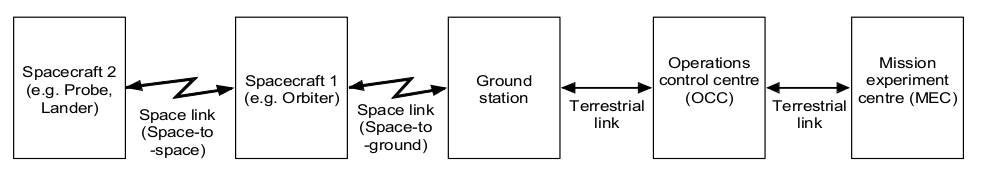
\includegraphics[scale=0.4]{fig/example_configuration_of_a_space_communication_system}
\caption{Example Configuration of a Space Communication System}
\label{fig:Example Configuration of a Space Communication System}
\end{figure}

A communications protocol is usually associated with one of the seven layers defined in the OSI Basic Reference Model. As in most terrestrial networks, protocols of the Session and Presentation Layers of the OSI model are rarely used over space links. Therefore the space link communications protocols are defined for the following five layers:

\begin{itemize}
\item Physical layer
\item Data Link layer
\item Network layer
\item Transport layer
\item Application layer
\end{itemize}

Figure \ref{fig:Space Communications Protocols Reference Model} shows the available space communications protocols and their associated layer.

\begin{figure}[h]
\centering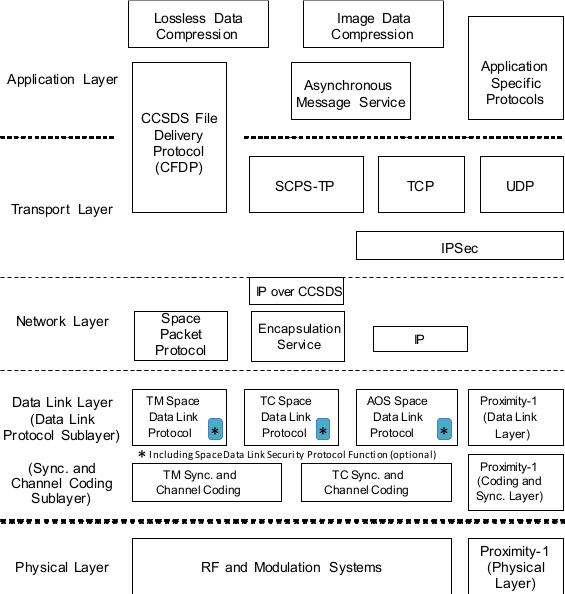
\includegraphics[scale=0.7]{fig/space_communications_protocols_reference_model}
\caption{Space Communications Protocols Reference Model}
\label{fig:Space Communications Protocols Reference Model}
\end{figure}

\subsubsection{Physical Layer}

\begin{tabular}{l}
\textit{CCSDS-401.0-B "Overview of Space Communications Protocols" \cite{CCSDS-401.0-B}} \\
\textit{CCSDS-413.0-G "Bandwidth-Efficient Modulations" \cite{CCSDS-413.0-G}} \\
\textit{ECSS-E-ST-50-05 "Space engineering - Radio frequency and modulation" \cite{ECSS-E-ST-50-05}}
\end{tabular}

The physical layer specification covers the characteristics of the radio frequency and modulation systems. It specifies the properties of the RF signals, namely the frequency stability, polarization, bandwidth occupations, and emissions, as well as the signal modulation (categorized into two categories: with residual carrier and with suppressed carrier). Further, link acquisition procedures and link budget calculations are defined.

\subsubsection{Data Link Layer}

\begin{tabular}{l}
\textit{CCSDS-130.2-G "Space Data Link Protocols--Summary of Concept and Rationale" \cite{CCSDS-130.2-G}}
\end{tabular}

The protocol data units used by the data link layer are called \textbf{transfer frames}. Each transfer frame consists of a header which provides protocol information and a data field within which \textbf{service data units} (SDU) are carried.

The sending of \textbf{telemetry} from a spacecraft to a ground station (the \textbf{return link}) uses fixed-length \textbf{telemetry transfer frames} (TMTF) to facilitate robust synchronization procedures over a noisy link. Their length is fixed on a particular physical channel and must be known to the receiving end before the actual reception occurs.

The sending of \textbf{telecommands} from ground to space (the \textbf{forward link}) uses variable-length \textbf{telecommand transfer frames} (TCTF) to facilitate reception of short messages with a short delay. The length of the frame is contained in its header. In order to notify the sender of TCTFs about the status of acceptance of TCTFs at the receiving end, another data unit called the communications link control word (CLCW) is embedded in the return link (i.e. in the telemetry). 

The mechanism used by the data link layer protocol for transferring data with different quality of service (QoS) requirements (mostly priority and latency) is the use of \textbf{virtual channels} (VC). The virtual channel concept allows one physical channel to be divided into multiple separate logical data channels, each identified by a virtual channel identifier (VCID). Each transfer frame transferred over a physical channel belongs to one of the virtual channels of the physical channel (see Figure \ref{fig:Virtual Channels}).

\begin{figure}[h]
\centering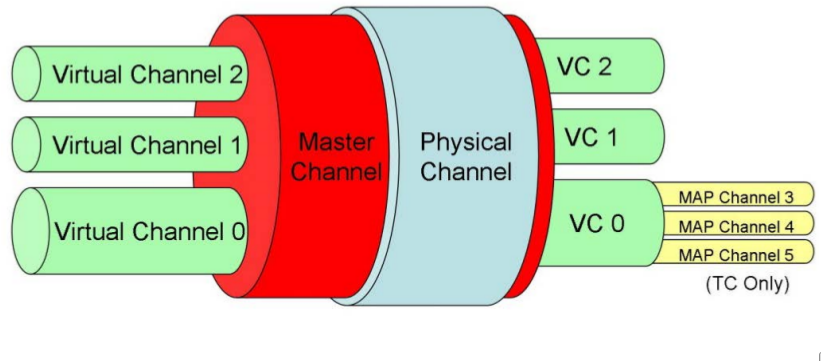
\includegraphics[scale=0.4]{fig/virtual_channels}
\caption{Virtual Channels}
\label{fig:Virtual Channels}
\end{figure}

\textbf{Telemetry Synchronization and Channel Coding Sublayer}

\begin{tabular}{l}
\textit{CCSDS-131.0-B "TM Synchronization and Channel Coding" \cite{CCSDS-131.0-B}} \\
\textit{CCSDS-130.1-G "TM Synchronization and Channel Coding--Summary of Concept and Rationale" \cite{CCSDS-130.1-G}}
\end{tabular}

The TM channel coding and synchronization sublayer provides the following three functions for transferring \textbf{telemetry transfer frames} over a space link: error-control coding, synchronization, and pseudo-randomization. 

For the \textbf{error-control coding} there are four coding types available: convolutional coding, Reed-Solomon coding, Turbo coding, and low-density parity-check coding. These coding schemes typically provide error detection and correction and are aimed for ensuring a reliable data transmission with low bit error rate over a channel with Gaussian noise. All of them however come at the price of complexity, and require a coder on the sending end and a decoder on the receiving end. The alternative is to use no coding at all, which may be acceptable depending on the link budget and the frame size. Figure \ref{fig:Telemetry Link Coding Options} shows the several coding options.

\begin{figure}[h]
\centering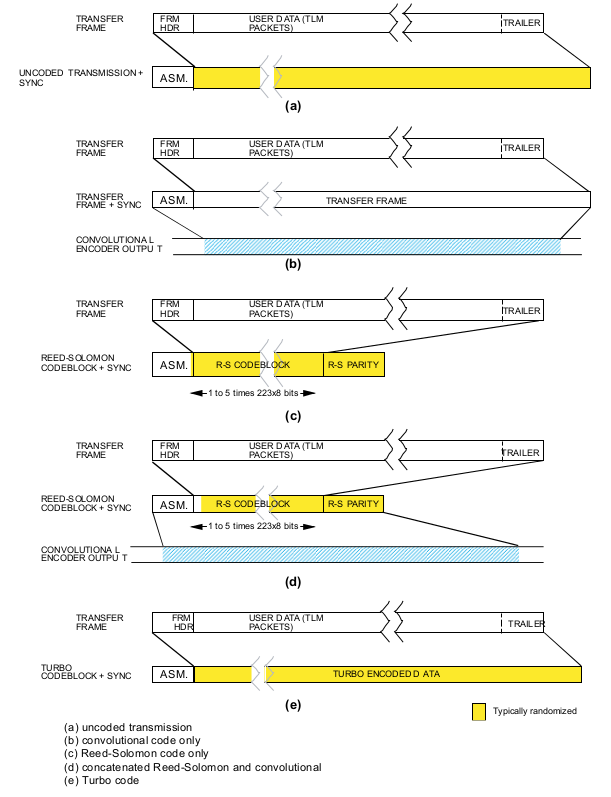
\includegraphics[scale=0.5]{fig/telemetry_link_coding_options}
\caption{Telemetry Link Coding Options}
\label{fig:Telemetry Link Coding Options}
\end{figure}

The \textbf{synchronization} of frames is necessary for the decoding process (if coding is applied) as well as for the pseudo-randomization. An \textbf{attached synch marker} (ASM) is used for this. The ASM is a 32 bit pattern that is fairly unique such that it can be recognized by the receiving end. The specific bit pattern represented in hexadecimal notation is 0x1ACFFC1D, transmitted from left to right. The ASM marks the start of the \textbf{channel access data unit} (CADU). A CADU is therefore defined as a ASM plus the coded or uncoded transfer frame. 

The transfer frame part of the CADU may optionally be exposed to \textbf{pseudo-randomization}. This is done to make the signal have sufficient bit transitions (i.e. avoid having long runs of zeros or ones), which is needed for the receiver to work properly. The pseudo-randomization process is fairly simple: the transfer frame is bitwise exposed to an XOR operation with a pseudo-random sequence, which is generated from the following polynomial: $h(x) = x^{8} + x^{7} +x^{5} + x^{3} + 1$. The sequence generator is initialized with all-ones at the start of each transfer frame.

There is no prescription on how to arrange the CADUs that are sent over the physical channel. Common practice is to send a continuous stream of CADUs back-to-back, and fill them with idle data if no data is available for insertion. A continuous stream of CADUs is essential for the ground receiving end if they only contain idle data, because each CADU also contains valuable information in the frame header and operational control field.

\textbf{Telecommand Synchronization and Channel Coding Sublayer}

\begin{tabular}{l}
\textit{CCSDS-231.0-B "TC Synchronization and Channel Coding" \cite{CCSDS-231.0-B}} \\
\textit{CCSDS-230.1-G "TC Synchronization and Channel Coding--Summary of Concept and Rationale" \cite{CCSDS-230.1-G}}
\end{tabular}

The TC channel coding and synchronization sublayer provides the following four functions for transferring \textbf{telecommand transfer frames} over a space link: error-control coding, synchronization, pseudo-randomization, and repeated transmissions. 

For the \textbf{error-control coding} a modified Bose-Chaudhuri-Hocquenghem (BCH) code is used to reduce the effects of noise in the physical layer and establish a reliable data channel. The BCH codeblock is a fixed-length data entity as shown in Figure \ref{fig:BCH Codeblock Format}. Note that the filler bit is appended to achieve an integer number of bytes per codeblock. It is always set to zero. 

\begin{figure}[h]
\centering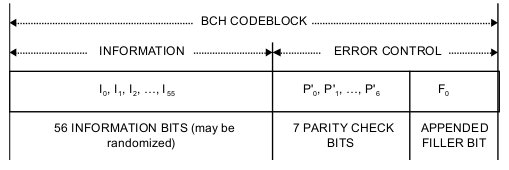
\includegraphics[scale=0.7]{fig/bch_codeblock_format}
\caption{BCH Codeblock Format}
\label{fig:BCH Codeblock Format}
\end{figure}

The parity check bits for each codeblock are generated from a polynomial $g(x) = x^{7} + x^{6} +x^{2} + 1$. It is initialized with all-zeros for each codeblock. Using the parity bits, the receiving end can decode in either error-detecting mode (triple error detection), or in an error-correcting mode (single error correction). 

To achieve \textbf{synchronization} the \textbf{communications link transmission unit} (CLTU) data structure is used. The CLTU is a data structure which carries data as continuous series of encoded BCH codeblocks. The data contained in the BCH codeblocks consist of one or more TC transfer frames from the sublayer above (possibly with fill data). The format of a CLTU is shown in Figure \ref{fig:CLTU Format}. 

\begin{figure}[h]
\centering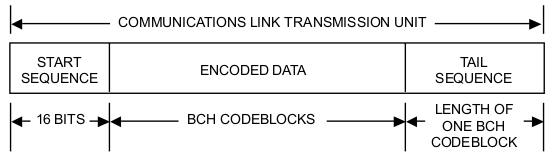
\includegraphics[scale=0.6]{fig/cltu_format}
\caption{CLTU Format}
\label{fig:CLTU Format}
\end{figure}

The start sequence of the CLTU delimits the start of the encoded data within the CLTU. The value of the start sequence in hexadecimal notation is 0xEB90. The encoded data consists of a set of BCH codeblocks, which may have been randomized or not. The tail sequence is a data structure which is constructed specifically to be a noncorrectable sequence which delimits the end of a CLTU by stopping the decoding process. The tail sequence consists of seven bytes of value 0xC5 and one byte with value 0x79. Alternatively the idle sequence consisting of eight bytes of value 0x55 is usable as well.

In order to maintain bit synchronization at the receiving end, the data stream must be sufficiently random. The transfer frame part of the CLTU may therefore optionally be exposed to \textbf{pseudo-randomization}. The pseudo-randomization process is fairly simple: the transfer frame is bitwise exposed to an XOR operation with a pseudo-random sequence, which is generated from the following polynomial: $h(x) = x^{8} + x^{6} +x^{4} + x^{3} + x^{2} + x + 1$. The sequence generator is initialized with all-ones at the start of each transfer frame.

In particular for long-distance links, it is common to send each CLTU with several \textbf{repetitions} in order to increase the likelihood of reception at the receiving end.

The procedure for sending CLTUs over the physical channel is named \textbf{physical layer operation procedure} PLOP. There are two options available, with PLOP-2 being the preferred one. It is defined as follows in terms of \textbf{carrier modulation modes} (CMM):

\begin{enumerate}
\item Begin of command session
\item (CMM-1) Unmodulated carrier only
\item (CMM-2) Carrier modulated with acquisition sequence
\item (CMM-3) Carrier modulated with one CLTU
\item (CMM-4) Carrier modulated with idle sequence 
\item Repeat from step 4 for each CLTU
\item (CMM-1) Unmodulated carrier only
\item End of command session
\end{enumerate}

The acquisition sequence and the idle sequence is a pattern of alternating ones and zeros, starting with either a one or a zero. The acquisition sequence shall be at least 128 bits (16 bytes) long and the idle sequence shall be at least 8 bits long.

\textbf{Telemetry Space Data Link Protocol Sublayer}

\begin{tabular}{l}
\textit{CCSDS-132.0-B "TM Space Data Link Protocol" \cite{CCSDS-132.0-B}} 
\end{tabular}

The telemetry space data link protocol has the features that it is: unidirectional (data flow is one way), unconfirmed service (sending end does not receive confirmation), incomplete service (completeness is not guaranteed), sequence-preserving (the sequence of service data units is preserved, although there may be gaps and duplications).

The telemetry transfer frame is composed of the mandatory and optional fields as shown in Figure \ref{fig:TM Transfer Frame Format}. Although the transfer frame data field is shown with undefined length, the length must be chosen and kept fixed over the mission phase for any channel. Figure \ref{fig:TM Transfer Frame Primary Header Format} shows the format of the primary header.

\begin{figure}[h]
\centering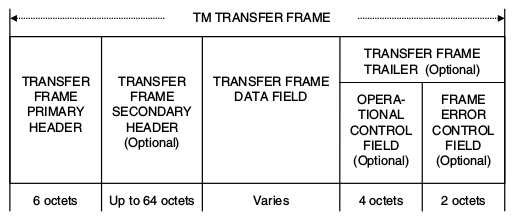
\includegraphics[scale=0.6]{fig/tm_transfer_frame_format}
\caption{TM Transfer Frame Format}
\label{fig:TM Transfer Frame Format}
\end{figure}

\begin{figure}[h]
\centering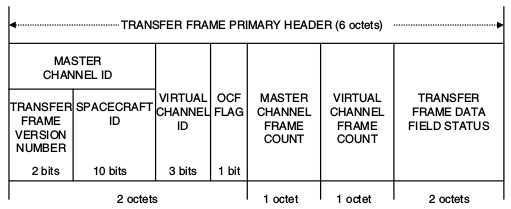
\includegraphics[scale=0.6]{fig/tm_transfer_frame_primary_header_format}
\caption{TM Transfer Frame Primary Header Format}
\label{fig:TM Transfer Frame Primary Header Format}
\end{figure}

The fixed-length TMTF is used to transport variable-length space packets (see Section \ref{sec:Network Layer}) as its service data unit. A TMTF may contain one, several, or zero space packets (in the later case it only contains idle data). Packets are concatenated and inserted into the TMTF until its length is exceeded. Any packet that exceeds the size of the TMTF data field will be split, and starts a new TMTF data field on the same virtual channel with its remainder. For the case where no Packets are available for inserting, idle data is written into the TMTF data field.

The TMTF primary header contains essential information about its source (spacecraft ID) and its channel properties. The data status field provides information about if and where a new packet starts in the data field.

The purpose of the operational control field (OCF) is to provide a mechanism for the retransmission control, namely the communications link control word, as defined in the following.

\textbf{Telecommand Space Data Link Protocol Sublayer}

\begin{tabular}{l}
\textit{CCSDS-232.0-B "TC Space Data Link Protocol" \cite{CCSDS-232.0-B}} \\
\textit{CCSDS-232.1-B "Communications Operation Procedure-1" \cite{CCSDS-232.1-B}}
\end{tabular}

The telecommand space data link protocol has the features that it is: unidirectional (data flow is one way), asynchronous service (data transfer is requested at any time), sequence preserving service (the sequence of service data units is preserved, except for expedited Type-B service).

The telecommand transfer frame is composed of the mandatory and optional fields as shown in Figure \ref{fig:TC Transfer Frame Format}. The transfer frame data field is of variable length. Figure \ref{fig:TC Transfer Frame Primary Header Format} shows the format of the primary header.

\begin{figure}[h]
\centering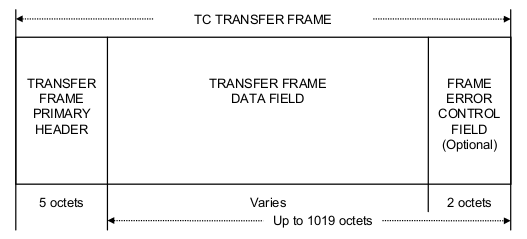
\includegraphics[scale=0.6]{fig/tc_transfer_frame_format}
\caption{TC Transfer Frame Format}
\label{fig:TC Transfer Frame Format}
\end{figure}

\begin{figure}[h]
\centering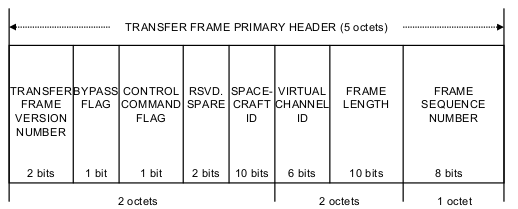
\includegraphics[scale=0.6]{fig/tc_transfer_frame_primary_header_format}
\caption{TC Transfer Frame Primary Header Format}
\label{fig:TC Transfer Frame Primary Header Format}
\end{figure}

The variable-length TCTF is used to transport variable-length space packets (see Section \ref{sec:Network Layer}) as its service data unit. A TCTF may contain one or several space packets. To improve system throughput efficiency, relatively small TCTFs are desirable. Therefore, large space packets are broken into smaller pieces via segmentation and sent in several consecutive TCTFs. On the other hand, very small space packets may be grouped together via blocking and transferred in a single TCTF.

The TCTF primary header contains essential information about its destination (spacecraft ID) and its channel properties. It contains a bypass and control command flag that are used to indicate how sequence control is applied to the frame and what data is contained in the data field:

\begin{itemize}
\item Type-AD: The data field carries space packets, subject to sequence control.
\item Type-BD: The data field carries space packets, bypassing sequence control.
\item Type-BC: The data field carries control commands, bypassing sequence control.
\end{itemize}
 
The transfer frame data field therefore may carry space packet data or control commands. For the case of transferring space packets, a \textbf{segment header} is inserted as the first byte of the data field, with the format defined in Figure \ref{fig:Segment Header Format}. Following the segment header are: a complete packet, multiple packets, or a portion of a packet (Figure \ref{fig:Blocking and Segmentation}). The sequence flags in the segment header are used to distinguish between these cases. Also, the segment header introduced yet another mechanism for further channel multiplexing. Namely it allows the definition of several \textbf{multiplexer access points} (MAP) to be used on a particular virtual channel.

\begin{figure}[h]
\centering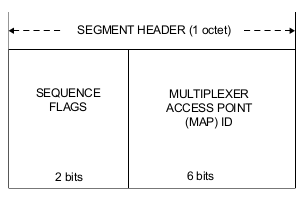
\includegraphics[scale=0.6]{fig/segment_header_format}
\caption{Segment Header Format}
\label{fig:Segment Header Format}
\end{figure}

\begin{figure}[h]
\centering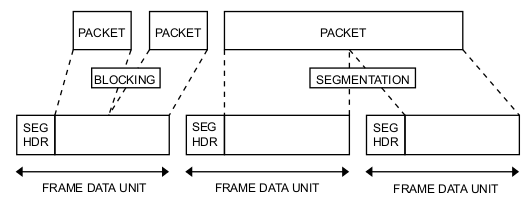
\includegraphics[scale=0.6]{fig/blocking_and_segmentation}
\caption{Blocking and Segmentation}
\label{fig:Blocking and Segmentation}
\end{figure}

For the case where the data field carries \textbf{control commands}, it may contain either  an unlock command, or a command for setting the receiver frame sequence number. These two commands are essential for controlling the sequence control mechanism of the uplink, which is realized through a procedure called communications operation procedure.

The \textbf{communications operation procedure} (COP) is a closed-loop procedure executed by the sending and receiving ends of the telecommand space data link protocol. COP utilizes an automatic request for retransmission (ARQ) procedure to retransmit transfer frames that were rejected by the receiving end. It ensures that Type-AD frames are only accepted at the receiving end in strict sequential order, without omission or duplication. 

COP-1 consists of a pair of synchronized procedures for each virtual channel: a \textbf{frame operation procedure} (FOP-1) at the sending end and a \textbf{frame acceptance and reporting mechanism} (FARM-1) at the receiving end. FOP-1 transmits telecommand transfer frames to the FARM-1 of the same virtual channel. The FARM-1 returns reports of the status of transfer frame acceptance to the FOP-1 using the \textbf{communications link control word} (CLCW), which is placed in the operational control field of a telemetry transfer frame. The format of a CLCW is shown in Figure \ref{fig:Communications Link Control Word Format}.

\begin{figure}[h]
\centering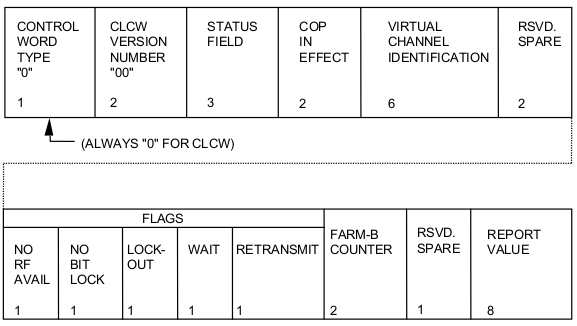
\includegraphics[scale=0.6]{fig/communications_link_control_word_format}
\caption{Communications Link Control Word Format}
\label{fig:Communications Link Control Word Format}
\end{figure}

The \textbf{sequence-controlled service} (also called AD service) is realized through the use of synchronized counters (see Figure \ref{fig: COP-1 Variables, Frame, and Report Values}). For each transmitted and received Type-AD telecommand transfer frame the counter increases on the sending and on the receiving end, respectively. Any loss of transfer frame would result in a mismatch of these counters and will immediately cause the rejection of further incoming telecommand frames.

\begin{figure}[h]
\centering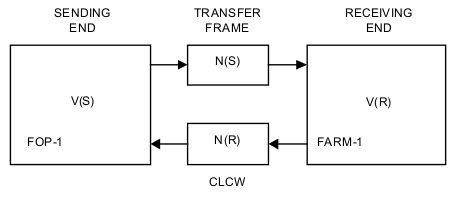
\includegraphics[scale=0.6]{fig/cop-1_variables_frame_and_report_values}
\caption{COP-1 Variables, Frame, and Report Values}
\label{fig: COP-1 Variables, Frame, and Report Values}
\end{figure}

The Type-BC transfer frames are used to carry control commands to configure COP-1, namely to handle locked out situations and to synchronize the counters.

Finally, the expedited service (BD service) is used only in exceptional circumstances, typically during spacecraft recovery. Here the frames are not subjected to sequence control and hence there is no guarantee that all are delivered.

\subsubsection{Network Layer}
\label{sec:Network Layer}

\begin{tabular}{l}
\textit{CCSDS-133.0-B "Space Packet Protocol" \cite{CCSDS-133.0-B}} 
\end{tabular}

The protocol data units used by the network layer are called \textbf{space packets}. Aside from a header that identifies the packet, the internal data content is completely under control of the user application.

The space packets protocol has the features that it is: pre-configured (user data can be sent only through pre-defined logical data path), unidirectional (data flow per defined path is one way), asynchronous (data transfer takes place at any time), unconfirmed service (sending end does not receive confirmation), incomplete service (completeness is not guaranteed), non-sequence-preserving (the sequence of service data units may not be preserved).

The space packet is composed of the fields as shown in Figure \ref{fig:Space Packet Format}. The packet data field is of variable length. Figure \ref{fig:Space Packet Primary Header Format} shows the format of the primary header. The optional packet secondary header may be used to transport time and/or other essential ancillary data in the same location within each and every space packet.

\begin{figure}[h]
\centering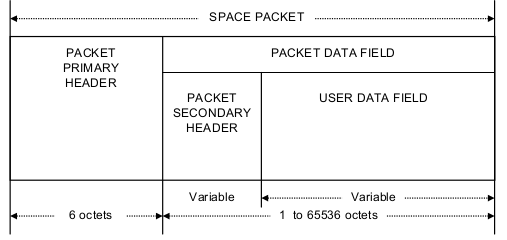
\includegraphics[scale=0.6]{fig/space_packet_format}
\caption{Space Packet Format}
\label{fig:Space Packet Format}
\end{figure}

\begin{figure}[h]
\centering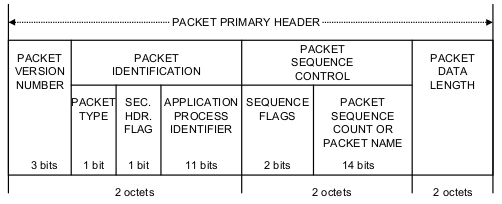
\includegraphics[scale=0.6]{fig/space_packet_primary_header_format}
\caption{Space Packet Primary Header Format}
\label{fig:Space Packet Primary Header Format}
\end{figure}

The \textbf{application process identifier} (APID) is a unique identifier for the sending or receiving application process. The APID is used to identify the \textbf{logical data path} of that particular packet, in order to allow the underlying subnetwork services to route the packet to its destination. 

\subsubsection{Space Link Protocol Stack}

The protocol stack for transport of telecommands and telemetry are shown in Figure \ref{fig:Telecommand Protocol Stack} and Figure \ref{fig:Telemetry Protocol Stack}.

\begin{figure}[h]
\centering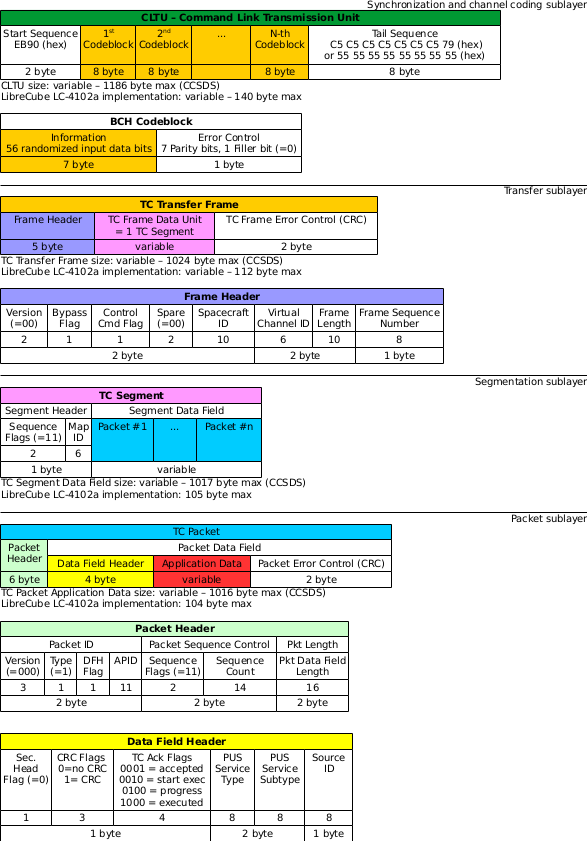
\includegraphics[scale=0.4]{fig/telecommand_protocol_stack}
\caption{Telecommand Protocol Stack}
\label{fig:Telecommand Protocol Stack}
\end{figure}

\begin{figure}[h]
\centering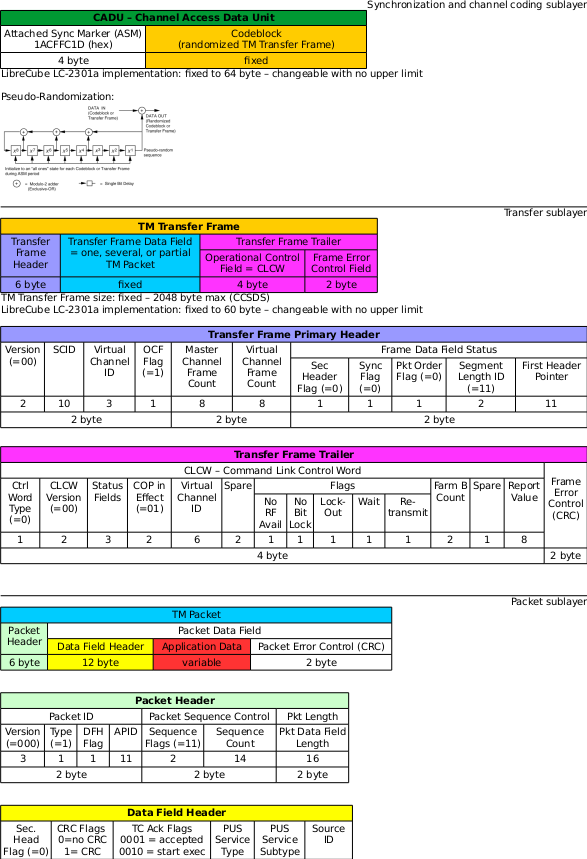
\includegraphics[scale=0.4]{fig/telemetry_protocol_stack}
\caption{Telemetry Protocol Stack}
\label{fig:Telemetry Protocol Stack}
\end{figure}

\clearpage
\subsection{Onboard Interface Services}

\begin{tabular}{l}
\textit{CCSDS-850.0-G "Spacecraft Onboard Interface Services" \cite{CCSDS-850.0-G}} 
\end{tabular}

The spacecraft onboard interface services (SOIS) standardizes the services to be supported by underlying protocols in the onboard software (OBSW) on application support layer and subnetwork layer. Figure \ref{fig:Spacecraft Onboard Interface Services Reference Model} shows a layered view of the recommended services and their associated access points. User, i.e. mission specific applications make use of the \textbf{application support layer} services (and possibly any lower level service). The \textbf{transfer layer} provides transport and network layer services based on existing (or dedicated) protocols (such as space packet for the network protocol). In many cases the transport layer will not be required, unless routing across multiple data links is needed. The \textbf{subnetwork layer} provides access to the data link medium and provides a set of services to be mapped over the subnetwork defined by that medium.

\begin{figure}[h]
\centering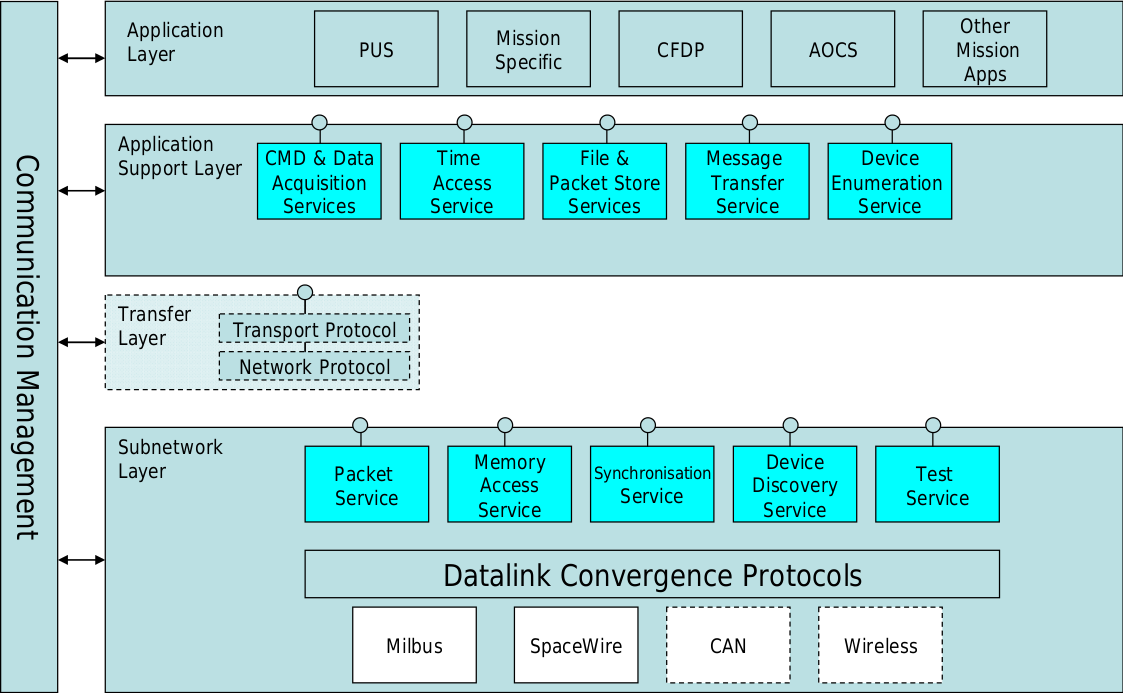
\includegraphics[scale=0.4]{fig/spacecraft_onboard_interface_services_reference_model}
\caption{Spacecraft Onboard Interface Services Reference Model}
\label{fig:Spacecraft Onboard Interface Services Reference Model}
\end{figure}


\subsubsection{Subnetwork Layer - Packet Service}

\begin{tabular}{l}
\textit{CCSDS-851.0-M "Spacecraft Onboard Interface Services--Subnetwork Packet Service" \cite{CCSDS-851.0-M}} 
\end{tabular}

The \textbf{packet service} transfers variable length, delimited octet strings from one endpoint on a data link to another endpoint within the same subnetwork. It defines four classes of quality of service (QoS) for the transfer and provides the following three primitives: packet send request, packet receive indication, and packet failure indication (depending on the QoS).

\subsubsection{Subnetwork Layer - Memory Access Service}

\begin{tabular}{l}
\textit{CCSDS-852.0-M "Spacecraft Onboard Interface Services--Subnetwork Memory Access Service" \cite{CCSDS-852.0-M}} 
\end{tabular}

The \textbf{memory access service} provides means for a user entity to retrieve or change data located in memory hosted by a node on a subnetwork. The QoS comprises acknowledgement, authorisation, priority, and other aspects. The service provides the following primitives: read request, read indication, write request, an atomic read/modify/write request (useful for example to set individual bits), and a memory access result indication (as a response to the write and atomic read/modify/write).

\subsubsection{Subnetwork Layer - Subnetwork Synchronisation Service}

\begin{tabular}{l}
\textit{CCSDS-853.0-M "Spacecraft Onboard Interface Services--Subnetwork Synchronisation Service" \cite{CCSDS-853.0-M}} 
\end{tabular}

The \textbf{synchronisation service} provides a means for a user entity to maintain knowledge of time which is common to all data systems on the subnetwork. It is a best-effort service which provides the following primitives: time request, time indication, and optionally also: event request, event indication.

\subsubsection{Subnetwork Layer - Subnetwork Device Discovery Service}

\begin{tabular}{l}
\textit{CCSDS-854.0-M "Spacecraft Onboard Interface Services--Subnetwork Device Discovery Service" \cite{CCSDS-854.0-M}} 
\end{tabular}

The \textbf{device discovery service} provides a means for a user entity to receive notification of the presence of other nodes on the subnetwork. It is a best-effort service which provides the following primitives: device discovery request, device discovery indication, and device discovery loss indication.

\subsubsection{Subnetwork Layer - Subnetwork Test Service}

\begin{tabular}{l}
\textit{CCSDS-855.0-M "Spacecraft Onboard Interface Services--Subnetwork Test Service" \cite{CCSDS-855.0-M}} 
\end{tabular}

The \textbf{test service} provides a means for a user entity to test functionality and connectivity of the subnetwork. It is a best-effort service, which provides the following primitives: test request and test indication.

\subsubsection{Application Support Layer - Command and Data Acquisition Services}

The \textbf{command and data acquisition services} provide the ability for onboard applications to command and acquire data from onboard devices across subnetworks, whilst being isolated from the protocols associated with the particular subnetworks. Applications can interface to the functionality directly provided by a physical device or with a higher level abstraction of the physical device, known as a virtual device. The individual services that comprise the command and data acquisition services are described in the following.

\begin{tabular}{l}
\textit{CCSDS-871.0-M "Spacecraft Onboard Interface Services--Device Access Service" \cite{CCSDS-871.0-M}} 
\end{tabular}

The \textbf{device access service} (DAS) provides a standard interface between onboard software applications and flight hardware such as sensors and actuators. To acquire a value (i.e. data) from a device, an application invokes the "acquire from device request" primitive and obtains the result in form of an "acquire from device indication" primitive. To command (i.e. send a value to) a device, an application invokes the "command device request" primitive and obtains the result in form of an "command device indication" primitive, which indicates whether or not the command was sent successfully and, if available, more result metadata. The DAS uses either the packet service or the memory access service form the subnetwork layer to implement its functionality. An example is shown in Figure \ref{fig:Example Device Access Service}.

\begin{figure}[h]
\centering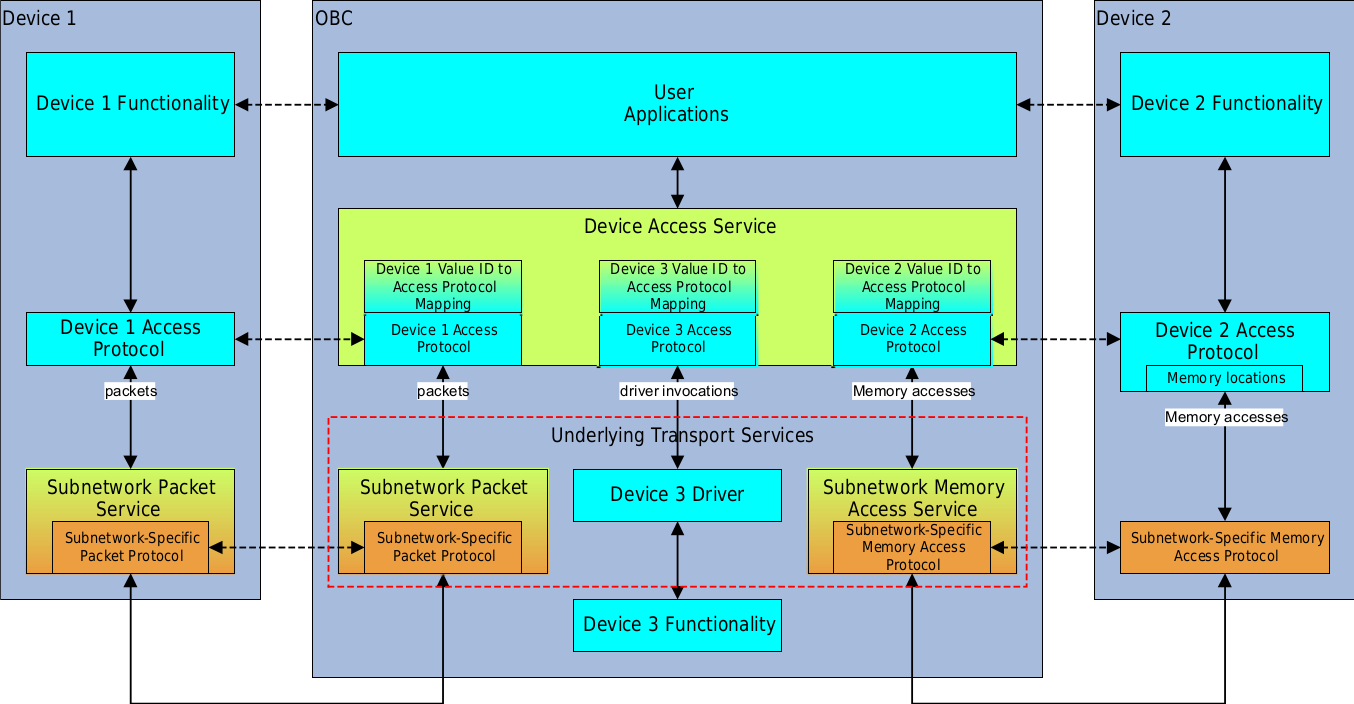
\includegraphics[scale=0.3]{fig/example_device_access_service}
\caption{Example Device Access Service}
\label{fig:Example Device Access Service}
\end{figure}

\begin{tabular}{l}
\textit{CCSDS-871.2-M "Spacecraft Onboard Interface Services--Device Virtualization Service" \cite{CCSDS-871.2-M}} 
\end{tabular}

The \textbf{device virtualization service} (DVS) provides applications with functional interfaces to devices, abstracted from the protocols used for accessing the devices and the data encodings used in those protocols. This is a further abstraction on top of the device access service that provides applications with raw interfaces to devices, only abstracted from the subnetwork protocols used for exchanging data with the devices. Similar to the DAS, the DVS provides service primitives for commanding and data acquisitions. In contrast however, it uses logical identifiers for the device and value identifiers, which are then mapped to the physical ones via a managed \textbf{device and value identifier resolution table}.

An example would be to command ON a virtual image of a GPS unit via the DVS, which then invokes a number of DAS functions to implement this functionality. the required mapping of identifiers for each service layer is shown in Figure \ref{fig:Mapping of Identifiers}.

\begin{figure}[h]
\centering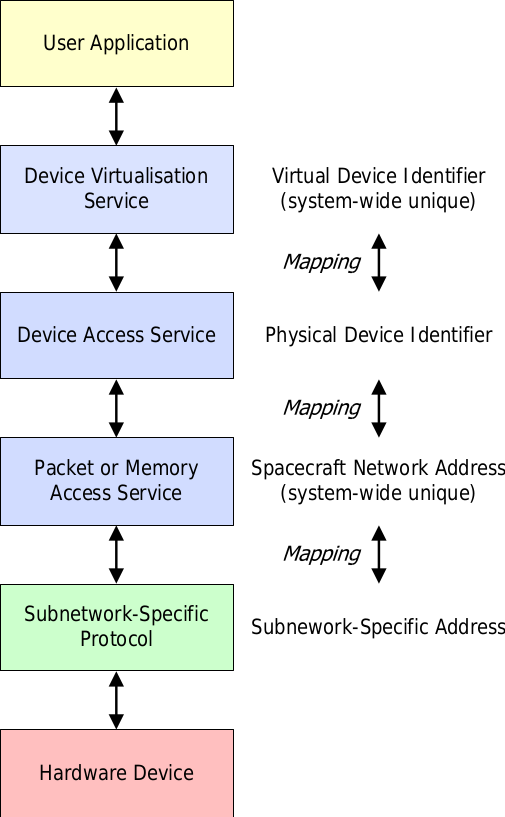
\includegraphics[scale=0.3]{fig/mapping_of_identifiers}
\caption{Mapping of Identifiers}
\label{fig:Mapping of Identifiers}
\end{figure}

\begin{tabular}{l}
\textit{CCSDS-871.1-M "Spacecraft Onboard Interface Services--Device Data Pooling Service" \cite{CCSDS-871.1-M}} 
\end{tabular}

The \textbf{device data pooling service} (DDPS) enables onboard software to access pooled data acquired from simple onboard hardware devices such as sensors and actuators, without explicitly requesting an acquisition from the real device. The layout of a data pool is shown in Figure \ref{fig:Layout of Data Pool}. At each sample acquisition, the various pre-defined values are sampled and stored together with a time stamp. A (normally short) history of those samples is maintained.

\begin{figure}[h]
\centering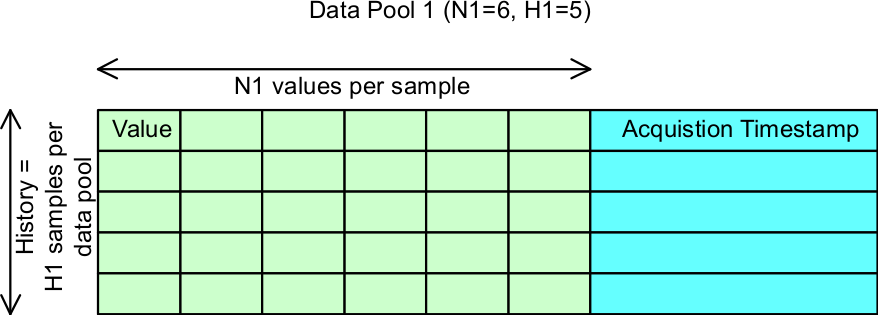
\includegraphics[scale=0.3]{fig/layout_of_data_pool}
\caption{Layout of Data Pool}
\label{fig:Layout of Data Pool}
\end{figure}

The sample acquisition period can be conveniently synchronized using the subnetwork synchronization service. This is shown in Figure \ref{fig:Example of Data Pooling Service}.

\begin{figure}[h]
\centering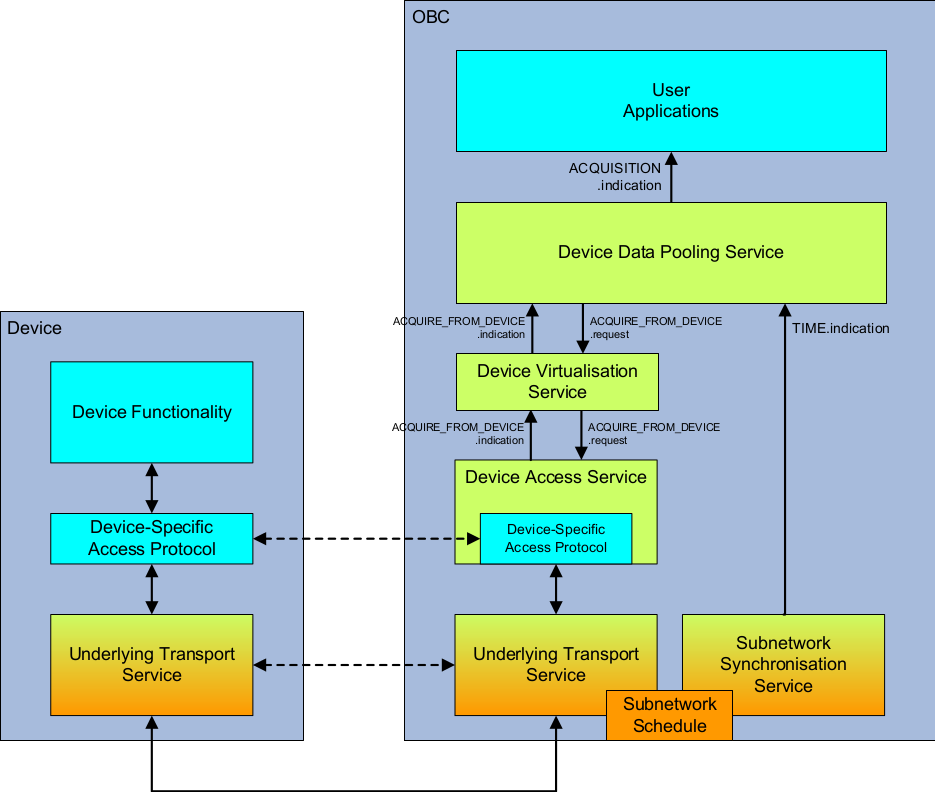
\includegraphics[scale=0.3]{fig/example_of_data_pooling_service}
\caption{Example of Data Pooling Service}
\label{fig:Example of Data Pooling Service}
\end{figure}

The DDPS provides service primitives for creating, deleting, starting, and stopping such data pools, and for reading them.

\begin{tabular}{l}
\textit{CCSDS-871.3-M "Spacecraft Onboard Interface Services--Device Enumeration Service" \cite{}} 
\end{tabular}

The \textbf{device enumeration service} (DES) provides management and user notification of addition of devices to or removal of devices from a spacecraft. The main goal of DES is to assist onboard reconfiguration functions, such as mode management or fault detection, isolation, and recovery regarding the notification of changes in the spacecraft configuration, and the execution of operations needed to adjust the onboard software to the new configuration. An example is given in Figure \ref{fig:Device Enumeration Service and Redundancy}.

\begin{figure}[h]
\centering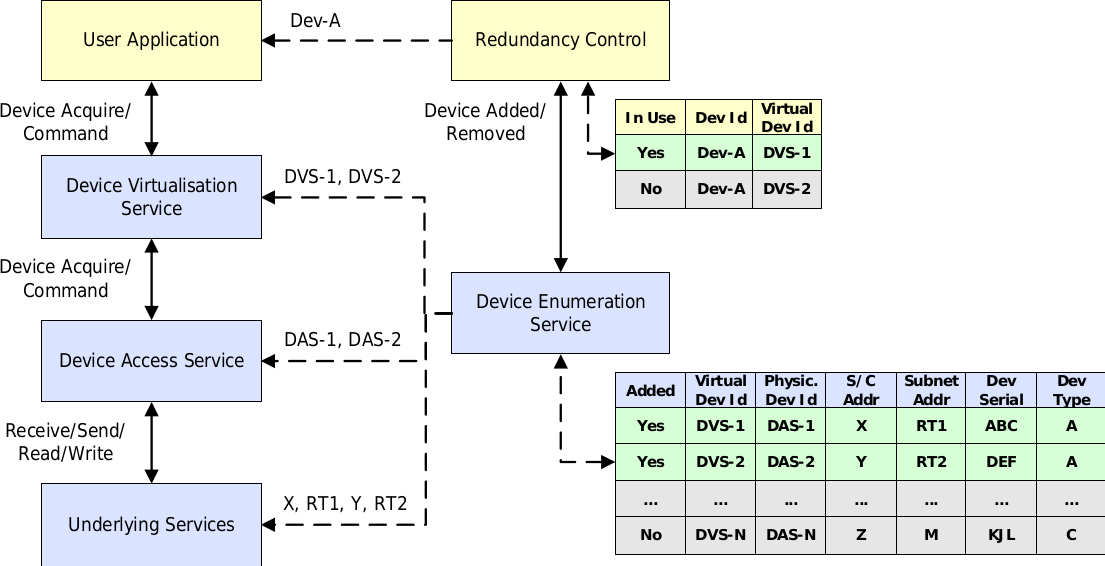
\includegraphics[scale=0.3]{fig/device_enumeration_service_and_redundancy}
\caption{Device Enumeration Service and Redundancy}
\label{fig:Device Enumeration Service and Redundancy}
\end{figure}

The DES provides service primitives for adding, removing, querying/enumerating of devices, and indications of devices found or lost. Its relationship with other SOIS services is shown in Figure \ref{fig:Relationship between Device Enumeration Service and other Services}.

\begin{figure}[h]
\centering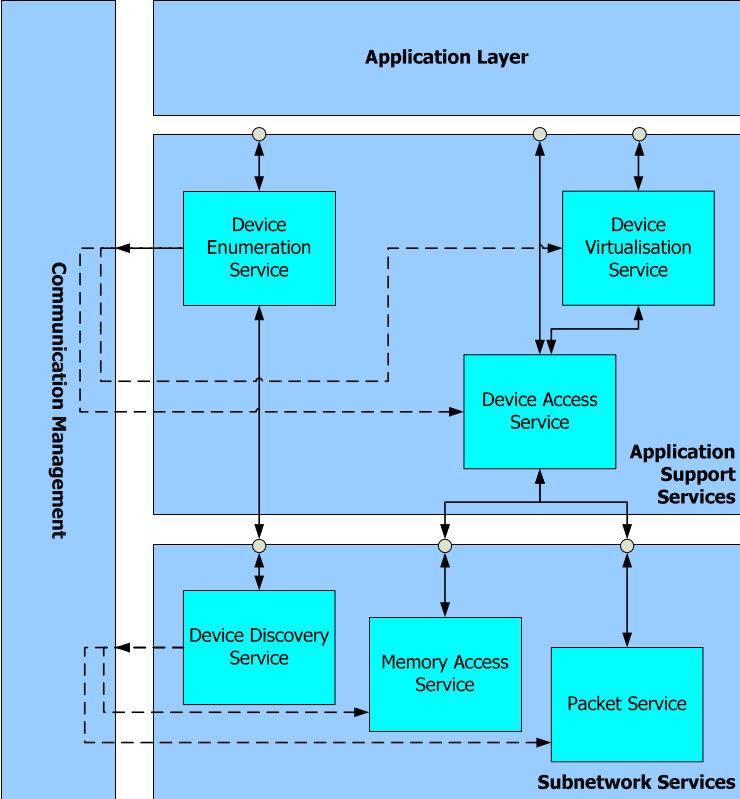
\includegraphics[scale=0.3]{fig/relationship_between_device_enumeration_service_and_other_services}
\caption{Relationship between Device Enumeration Service and other Services}
\label{fig:Relationship between Device Enumeration Service and other Services}
\end{figure}

\subsubsection{Application Support Layer - Time Access Services}

\begin{tabular}{l}
\textit{CCSDS-872.0-M "Spacecraft Onboard Interface Services--Time Access Service" \cite{}} 
\end{tabular}

The \textbf{time access service} provides a user entity with a consistent interface to a local time source that is correlated to some centrally maintained master onboard time source. The local time sources are typically free-running hardware counters accumulating seconds and sub-seconds of elapsed time. The master time source usually has the most accurate precision and broadcasts its time information to the other entities on the subnetwork, via the synchronisation service (see Figure \ref{fig:Typical Onboard Time System Architecture}). 

\begin{figure}[h]
\centering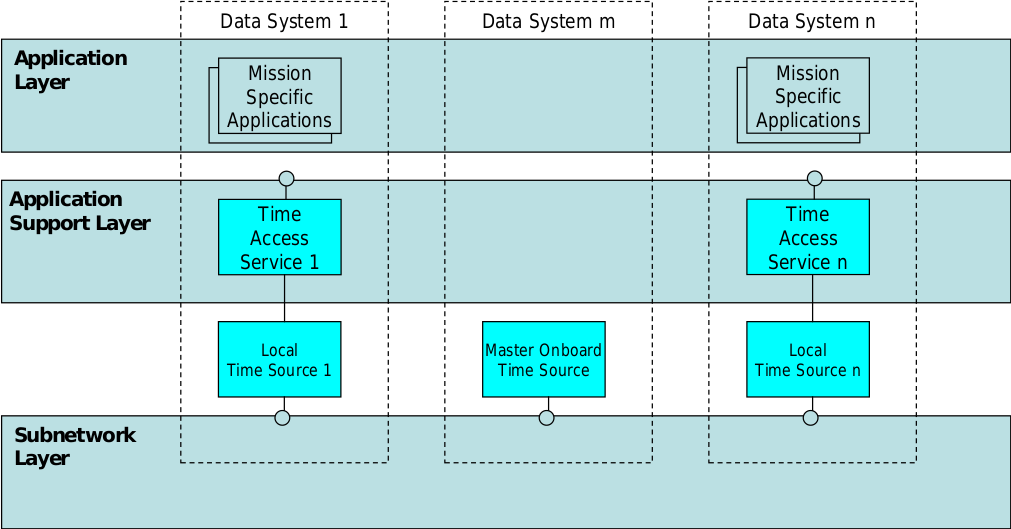
\includegraphics[scale=0.3]{fig/typical_onboard_time_system_architecture}
\caption{Typical Onboard Time System Architecture}
\label{fig:Typical Onboard Time System Architecture}
\end{figure}

Applications should use this service to obtain the time from the local time source rather than, for example, reading directly from the local elapsed time counter hardware registers. The service primitives provide are: time request and time indication for the so-called wall clock capability, and optionally, various primitives for implementing the alarm clock and metronome capability. 

\subsubsection{Application Support Layer - File and Packet Store Services}

\begin{tabular}{l}
\textit{CCSDS-873.0-M "Spacecraft Onboard Interface Services--Time Access Service" \cite{}} 
\end{tabular}

The \textbf{file and packet store services} (FPSS) comprise the following services: file access service (FAS), file management service (FMS), packet store access service (PSAS), and packet store management service (PSMS). These services are used to access and manage files and packets residing in file and packet stores. A \textbf{file store} is considered to be a file system (flat or hierarchical) and the associated storage medium. A \textbf{packet store} does not use a file system, but instead is organized either as an bounded or circular first-in first-out (FIFO) store, or a random-access store (the later being much more complex to manage). A large number of primitives are defined for each service to provide the functionality of accessing and managing the contents of the stores. An example deployment is shown in Figure \ref{fig:Example Deployment of Packet Store} where packets are stored in the onboard solid state mass memory (SSMM).

\begin{figure}[h]
\centering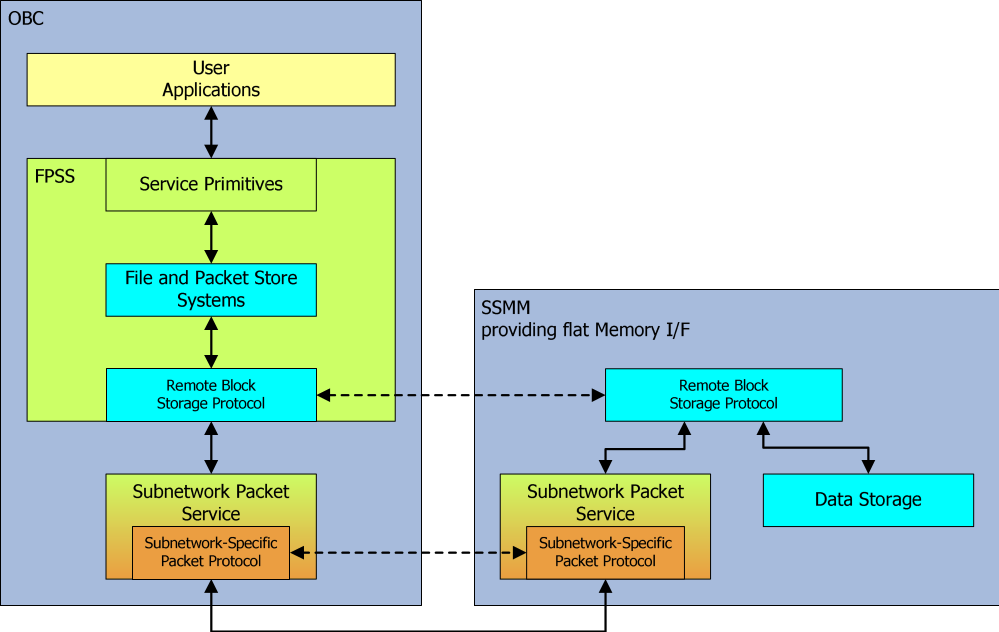
\includegraphics[scale=0.3]{fig/example_deployment_of_packet_store}
\caption{Example Deployment of Packet Store}
\label{fig:Example Deployment of Packet Store}
\end{figure}

\subsubsection{Application Support Layer - Message Transfer Service}

\begin{tabular}{l}
\textit{CCSDS-875.0-M "Spacecraft Onboard Interface Services--Message Transfer Service" \cite{}} 
\end{tabular}

The \textbf{message transfer service} (MTS) provides applications with a standard service for mediating the transfer of discrete data, i.e. messages, between onboard software users in a (potentially) distributed onboard system.

Four different models of message transfer exist:
\begin{itemize}
\item Send/receive: Messages may simple be sent to designated modules.
\item Synchronous query: Messages may be sent asynchronously but allowing synchronization with the message reply.
\item Publish/subscribe: Messages may be published to a time-varying number of self-selected subscribers.
\item Announcement: Messages may be sent to a set of modules selected by the message source.
\end{itemize}

The SOIS MTS is essentially a subset of the asynchronous message service (AMS). It provides a large number of service primitives with tailoring in respect to the MTS service definition.

\subsubsection{Electronic Data Sheets}

\begin{tabular}{l}
\textit{CCSDS-876.0-R "Spacecraft Onboard Interface Services--XML Specification for Electronic Data Sheets for Onboard Devices" \cite{}} \\
\textit{CCSDS-876.1-R "Spacecraft Onboard Interface Services--Common Dictionary of Terms for Onboard Devices and Software Components" \cite{}}
\end{tabular}

The \textbf{SOIS electronic datasheets} (SEDS) are intended to be a machine-understandable mechanism for describing devices which may be accessed using the SOIS command and data acquisition services. In this way it potentially shall replace the traditional user manuals, interface control documents, and datasheets which accompany a device and are necessary to determine the operation of the device and how to communicate with it.

The SEDS describes the format of information in a data interface for an onboard device accessed using the command and data acquisition service of the application support layer and the packet and memory access service of the subnetwork layer.

The SEDS are in XML format and specified by an XSD schema that allows for checking correct syntax. In addition, there is also a dictionary of terms (DoT) defined, which provides for semantic correctness checking. 

\subsection{Onboard Software Applications}
\label{sec:Onboard Software Applications}

\subsubsection{File Exchange Applications}

\begin{tabular}{l}
\textit{CCSDS-727.0-B "CCSDS File Delivery Protocol (CFDP)" \cite{CCSDS-727.0-B}} \\
\textit{CCSDS-720.1-G "CCSDS File Delivery Protocol (CFDP) Part 1: Introduction and Overview" \cite{CCSDS-720.1-G}} \\
\textit{CCSDS-720.2-G "CCSDS File Delivery Protocol (CFDP) Part 2: Implementers Guide" \cite{CCSDS-720.2-G}} \\
\end{tabular}

This standard defines a protocol suitable for the transmission of files to and from spacecraft data storage and capable of operating in a wide variety of mission configurations. In addition to the purely file delivery related functions, the protocol includes file management services to allow control over the storage medium. Although the protocol can operate over a wide range of subnetwork services, this standard assumes the use of existing CCSDS packet services. 

The CFDP enables the moving of a file from one filestore to another, where the two filestores are in general resident in separate data systems and often with an intervening space link. In its simplest form, the protocol provides a Core file delivery capability operating across a single link. For more complex mission scenarios, the protocol offers extended operation providing store-and-forward functionality across an arbitrary network, containing multiple links with disparate availability, as well as subnetworks with heterogeneous protocols (Figure \ref{fig:CCSDS File Delivery Protocol}).

\begin{figure}[h]
\centering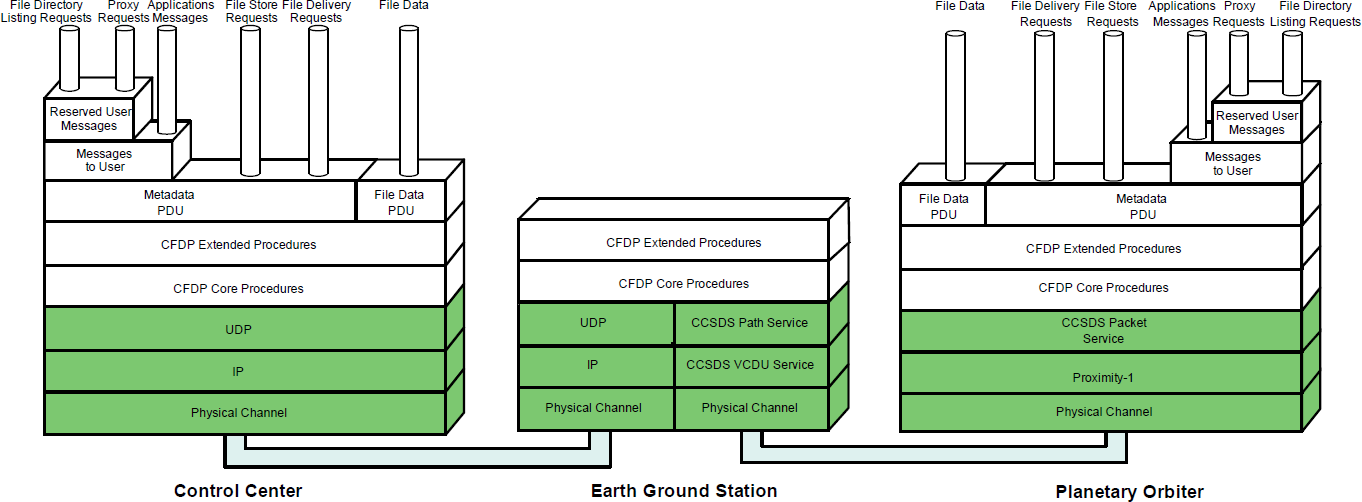
\includegraphics[scale=0.4]{fig/cfdp}
\caption{CCSDS File Delivery Protocol}
\label{fig:CCSDS File Delivery Protocol}
\end{figure}

\subsubsection{Packet Utilization Services}

\begin{tabular}{l}
\textit{ECSS-E-ST-70-41 "Telemetry and telecommand packet utilization" \cite{ECSS-E-ST-70-41}} \\
\end{tabular}

The packet utilization standard (PUS) addresses the utilization of telecommand packets and telemetry packets for the purposes of remote monitoring and control of spacecraft subsystems and payloads. It is defining the application level interface between ground and space, in order to satisfy the requirements of electrical integration and testing and flight operations.

The services defined by PUS cover a wide spectrum of operational scenarios and, for a given mission, only a subset of these services is likely to be appropriate. The PUS should be viewed as a "Menu" from which the applicable services and service levels are selected for a given mission. The specification of PUS services is adapted to the expectation that different missions require different levels of complexity and capability from a given service. 

The standardized PUS services fulfill the following criteria:
\begin{itemize}
\item Commonality: each standard service corresponds to a group of capabilities applicable to many missions.
\item Coherence: the capabilities provided by each standard service are closely related and their scope is unambiguously specified. Each standard service covers all the activities for managing interrelated state information and all activities that use that state information.
\item Self-containment: each standard service has minimum and well-defined interactions with other services or on-board functions.
\item Implementation independence: the standard services neither assume nor exclude a particular spacecraft architecture (hardware or software).
\end{itemize}

The standard service types are shown in Figure \ref{fig:PUS Services}. They include:

\begin{itemize}
\item Service types that provide basic functions such as collecting parameter statistics.
\item Service types that hold requests and release them to another service as appropriate. The time-based scheduling, the position-based scheduling and the event-action service types are examples of service types that hold and release requests following the occurrences of specified events.
\item Service types that provide standardized interfaces, for example to onboard devices, to an onboard control procedure engine or to an onboard file handling system.
\end{itemize}

\begin{figure}[h]
\centering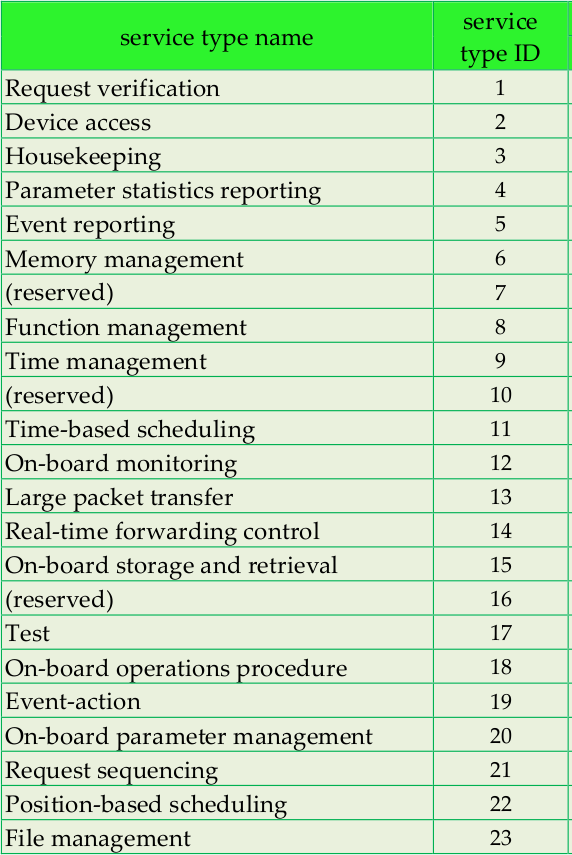
\includegraphics[scale=0.5]{fig/pus_services}
\caption{PUS Services}
\label{fig:PUS Services}
\end{figure}

When applying the PUS standard, a mission instantiates this standard by tailoring it for their needs. That instantiation results in a mission-specific packet utilization definition document that is rendered applicable to all partners involved in that mission. This document contains the mission-specific service type model that includes all PUS standardized service types considered suitable for use by that mission, each one tailored according to the mission needs, and all mission-specific additional service types.

\subsubsection{Onboard Control Procedures}

\begin{tabular}{l}
\textit{ECSS-E-ST-70-01 "Spacecraft on-board control procedures" \cite{ECSS-E-ST-70-01}} \\
\end{tabular}

The onboard control procedure (OBCP) concept is that of a procedure to be executed onboard, which can easily be loaded, executed, and also replaced, onboard the spacecraft without modifying the remainder of the onboard software. 

The benefits of implementing traditional onboard software (OBSW) functions as OBCPs include:
\begin{itemize}
\item the relative ease of development and validation of OBCPs vs. OBSW;
\item the core OBSW can be made more generic and is hence potentially reusable across many missions, if mission-specific functions are implemented as OBCPs; 
\item simplification of the OBSW maintenance task, i.e. changes to OBCPs can be easily and safely performed without changing the core OBSW. 
\end{itemize}

The availability of OBCPs enables operations procedures (both for routine functions and contingency operations) to be executed onboard as an alternative to on the ground (either  under manual control or automated in the mission control system). This can streamline the operations (reduction of bandwidth, potential reduction in operations manpower, reduction in  the loop delay inherent in ground control, simplification of ground procedures) as well as increasing their overall reliability. The use of  OBCPs also enhances the onboard autonomy capabilities and increases the robustness to ground station outages. 

